\documentclass[12pt]{article}
\usepackage[utf8]{inputenc}
\usepackage{amsmath}
\usepackage{amsfonts}
\usepackage{amssymb}
\usepackage{graphicx}
\usepackage{hyperref}
\usepackage{xspace}

%\graphicspath{{figures/}}
\usepackage{color}

\newcommand{\enm}[1]{\ensuremath{#1}\xspace}
\newcommand{\Rset}{\enm{\mathbb{R}}}
\newcommand{\vect}[1]{\enm{\boldsymbol{\mathbf{#1}}}}
\newcommand{\mat}[1]{\enm{\boldsymbol{\mathbf{#1}}}}

%%%%%%%%%%%%%%%%%%%%%%%%%%%%%%%%%%%%%%%%%%%%%%%%%%%%%%%%%%%%%%%%%%%%%
\begin{document}
\title{Test case for the UP4 2017-18 \\ 
Identification of a volcano reservoir from surface displacements
}
\author{Rodolphe Le Riche, Victor Picheny, Valérie Cayol}
%\date{15 february 2017}
\maketitle

\tableofcontents

\section{Foreword}
This directory contains data files with measured displacements at the surface of the Piton de la Fournaise volcano, along with files for modeling the displacements created by a specific magma reservoir. The source files are written in the R programming language. 
By matching the modeled and measured displacements, one can identify the reservoir underneath the volcano.
The test case was originally developped by Valérie Cayol, a volcanologist at CNRS, and re-implemented as an illustration for the course \cite{durrande:cel-01618068}. 
An illustration of the test case is provided in Figure~\ref{fig-piton}.
\begin{figure}
\begin{center}
\begin{minipage}{0.70\textwidth}
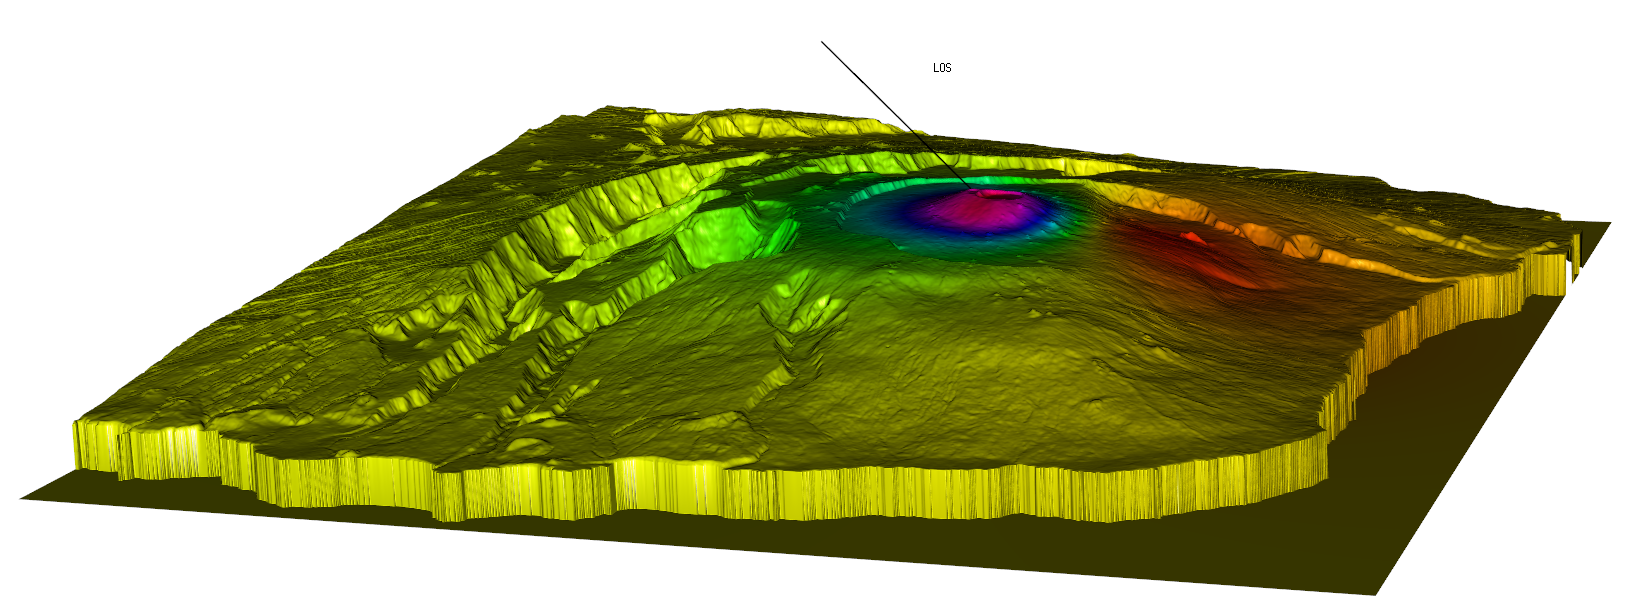
\includegraphics[width=\textwidth]{piton_ulos_2.png}
\end{minipage}
\hspace{0.05cm}
\begin{minipage}{0.44\textwidth}
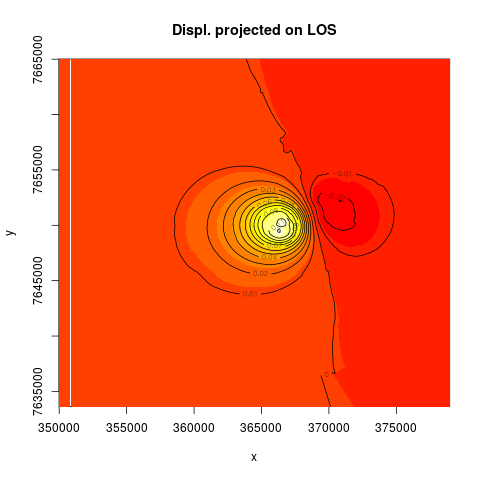
\includegraphics[width=\textwidth]{contour_ulos.png}
\end{minipage}
\end{center}
\caption{Digital terrain of the Piton de la Fournaise with displacements projected along the line of sight as colors (top) 
and (bottom) contour plot of the projected displacements (versus longitude $x$ and latitude $y$). 
These projected displacements are the quantities to match in order to estimate the magma reservoir.}
\label{fig-piton}
\end{figure}

\section{General test case presentation}
\subsection{General formulation}
The magma reservoir is the source of displacements at the surface of the volcano. 
The reservoir is assumed to have a spherical shape. It is described by $n=5$ inputs:
\begin{itemize}
\item The position of the center of the sphere
\begin{itemize}
\item the longitude and latiture in UTM meters, $x^S$ and $y^S$, respectively,
\item the elevation of the source with respect to sea level in meters, $z^S$,
\end{itemize}
\item the source radius in meters, $a$,
\item and the source overpressure in MPa, $p$.
\end{itemize}
These 5 scalars are the unknowns, or variables, of our problem and will be gathered in the 
vector $\vect{\theta} \in [\vect{\theta}^{min} , \vect{\theta}^{max}] \subset \Rset^5$.

The volcano displacements are seen by InSAR radars mounted on a satellite as the projection of the displacements along a line of sight (LOS).
Let $u_{LOS}(x,y;\vect{\theta})$ be the modeled displacement field parameterized by longitude and latitude $x$ and $y$,
\begin{equation}
\begin{split}
u_{LOS}(;\vect{\theta}):~ & \Rset^2 \rightarrow \Rset \\
 & (x,y) \mapsto u_{LOS}(x,y;\vect{\theta})
\end{split}
\label{eq-ulos}
\end{equation}
$u_{LOS}(;\vect{\theta})$ is expressed with the Mogi model \cite{Yamakawa1955,Mogi1958} which simulates the displacements created 
by a spherical magma chamber at the surface of a digital terrain.
The displacements are measured at a finite set of $m$ measurements points, $(x^i,y^i)$, which yields $u_{LOS}^\text{meas}(x^i,y^i)$, $i=1,\ldots,m$.
A weighted least squares distance between the measured and modeled displacements is expressed as
\begin{equation}
J_W^2(\vect{\theta}) ~=~ \frac{1}{2} \left( \vect{u_{LOS}^\text{meas}} - \vect{u_{LOS}(\vect{\theta})}\right)^\top \mat{W} \left( \vect{u_{LOS}^\text{meas}} - \vect{u_{LOS}(\vect{\theta})}\right) ~,
\label{eq-wls}
\end{equation}
where the bold face version of $u_{LOS}$ denotes its vectorized version at the measured points, e.g.,
\begin{equation*}
\vect{u_{LOS}(\vect{\theta})} ~=~ \left[ u_{LOS}(x^1,y^1;\vect{\theta}) \ldots u_{LOS}(x^m,y^m;\vect{\theta}) \right]^\top
\end{equation*}
and \mat{W} is a \emph{given} weight matrix, typically the inverse of a covariance matrix.


\paragraph{Normalizing a weighted least squares:} the distribution of $J^2_W(\vect{\theta})$ when \vect{\theta} is random within 
$[\vect{\theta}^{min} , \vect{\theta}^{max}]$ is far from being gaussian as it is bounded above 0 and has many very large 
values. The transformation $\log(1+J^2_W(\vect{\theta}))$ makes it more gaussian and will be used in the following as it makes 
the function more compatible with a gaussian process model.


\paragraph{Model identification as an optimization problem:} 
Finding the magma reservoir that corresponds to the measurements \vect{u_{LOS}^\text{meas}} amounts to minimizing 
the weighted least squares distance between the measurements and the Mogi model over the reservoir unknowns,
\begin{equation}
\vect{\theta}^\star  ~=~ \arg \min_{\vect{\theta} \in [\vect{\theta}^{min} , \vect{\theta}^{max}]} J^2_W(\vect{\theta})~.
\label{eq-minwls}
\end{equation}
In the case of ill-posed problems, the solution $\vect{\theta}^\star$ may not be unique. 

\vskip\baselineskip
To sum up, this project aims at learning (a normalized version of) the $n$ dimensional function $J^2_W(\vect{\theta})$ 
by carrying out a design of experiments (DoE), building a Gaussian process conditioned by the results of the DoE, and using it 
to minimize $J^2_W(\vect{\theta})$.

	\subsection{Installation, files provided and first steps}
	\subsubsection{Software prerequisites}
	\begin{enumerate}
	\item Have R available on your computer, cf. \url{https://www.r-project.org/}
	\item Optionally (but really helpful) have rstudio installed, cf. \url{https://www.rstudio.com}
	\item Install the ``R.matlab'' package to load the data that are in matlab format (\texttt{file\_name.mat}), 
	either from Tools / Install Package in rstudio or with the command \texttt{install.packages("R.matlab")}. 
	\item As above, install the following Dice suite of packages: ``DiceKriging'', ``DiceOptim'', ``DiceView''.
	\end{enumerate}

	\subsubsection{Files list}
	\begin{itemize}
	\item data files
	\begin{itemize}
	\item \texttt{fullgrid\_xyzulos.csv} : full digital terrain ($(x,y,x)$'s) and measured projected displacements in the ascii comma separated value format. Large file, only used for the plot demo (file \texttt{plots\_3d\_full\_grid.R}).
	\item \texttt{data\_nonoise.mat} : 220 measured $(x,y,x)$'s and associated $u_{LOS}$'s. Matlab format. Read and processed in the file 
	\texttt{mainScript\_DatascienceClass.R}.
	\end{itemize}
	\item R source files:
	\begin{itemize}
	\item \texttt{plots\_3d\_full\_grid.R}~: Loads the full digital model of the volcano (\texttt{fullgrid\_xyzulos.csv}), make a 3D plot of it, makes 2D contour maps of the displacements (target and another vector of variables).
	\item \texttt{mainScript\_DatascienceClass.R}~: utilities to load the data, and creates the function \texttt{compute\_wls} which calculates a 
	normalized $J^2_W$ (Eq.~\ref{eq-wls}).
	\item \texttt{wls\_ulos.R}~: calculates the weighted least squares distance $J^2_W$ (Eq.~\ref{eq-wls}) between the model projected displacements and the target.
	\item \texttt{mogi\_3D.R}~: calculate displacements on a digital terrain model from a point-wise spherical source.
	\item \texttt{kernels.R} contains utilities to build covariance functions and matrices, used here only to generate the \mat{W} weight matrix of Eq.~\ref{eq-wls}.
	\end{itemize}
	\item documentation: file \texttt{volcan\_test\_case.pdf}, compiled from \texttt{volcan\_test\_case.tex}, \texttt{biblio\_paper.bib}, 
	\texttt{contour\_ulos.png} and \texttt{piton\_ulos\_2.png}.
	\end{itemize}

	\begin{center}
	\fbox{
	\begin{minipage}{\textwidth}
\textbf{During the project, you should only use the function \texttt{compute\_wls} and should not change the rest of the provided code. }
\end{minipage}
}
\end{center}

\subsubsection{Running the demo step by step}
\begin{enumerate}
\item Open with rstudio the file \texttt{plots\_3d\_full\_grid.R} and ``source'' it, or start R in a console in the file directory and type
\texttt{source("plots\_3d\_full\_grid.R")}. 
A 3D window opens that shows the digital terrain of the volcano with a color projection of the displacements to be identified ($\vect{u_{LOS}^\text{meas}}$). The line of sight is drawn at the top of the volcano. The 3D plot can be rotated. 
Contours plots are also given, where new set of variables \vect{\theta} can be tried and compared through their $\vect{u_{LOS}(\vect{\theta})}$ to the targeted variables.
\item Open in rstudio the file \texttt{mainScript\_DatascienceClass.R}, or open the file with any text editor and start R in a console. 
The code is split in parts separated by a line of comments (\verb=#### step #####... =).
The first part loads libraries and utility files (e.g., the one coding the Mogi model).
The second part provides the variables bounds $\vect{\theta}^{min}$ and $\vect{\theta}^{max}$ (encoded as \texttt{xmin} and \texttt{xmax}) along with other variables related data.
The third part (\verb=#### load data #####... =) loads the data, in particular the location of the measurements, $(x^i,y^i)$ as \texttt{Glb\_xi} and \texttt{Glb\_yi}, and the vector of measured displacements as \texttt{Glb\_ulos}.
The fourth and last part provides functions for norming and unnorming the variables and norming the weighted least squares ($J^2_W$). It finishes with \texttt{compute\_wls <- function(x)} whose input \texttt{x} is \vect{\theta} and whose output is a normalized and centered $\log(1 + J^2_W(\vect{\theta}))$.
\end{enumerate}

\subsubsection{Overall goal of the project}
From that point onwards, it will be your goal to complete the code, mainly using DiceKriging and DiceOptim to 
\begin{enumerate}
\item build a statistical model of the function \texttt{compute\_wls} (the normalized $\log(1 + J^2_W(\vect{\theta}))$),
\item validate it,
\item minimize it and
\item analyze the results
\end{enumerate}
following the detailed instructions of each session.

\section{Building a kriging model of the weighted least squares function (WLS)}
%{\color{red}Victor, Olivier, Andres}
%\subsection{Make a design of experiments}
%\subsection{Scale the output}
%\subsection{Choose a Gaussian process kernel and learn it}
%\subsection{Test the Gaussian process}

Cf. text of ``TP1 : plans remplissant l’espace et krigeage'' by Victor Picheny.

\section{Identification of the volcano source}
%{\color{red}Rodolphe}
The goal of the practical session is to estimate solutions to the identification problem of Eq.~(\ref{eq-minwls}).
Because in real world situations, a call to the volcano model (through the \texttt{wls\_ulos} function) would be
computationally expensive, we will use the EGO algorithm \cite{Jones1998} in its DiceOptim version.
\begin{enumerate}
\item Write a script where the function \texttt{EGO.nsteps} is called with \texttt{compute\_wls} as objective function. 
\item Plot the results: \texttt{res\$value} to look at the convergence of the objective function, \texttt{pairs(res\$lastmodel@X)},
to look at the distribution of the points in the DoE (look at the best points and at the points added), 
\texttt{hist(res\$value)} to look at the distribution of objective functions sampled by EGO.
\item Comment on the distribution of the best reservoir variables.
\end{enumerate}


%\section{Global sensitivity analysis of the variables}
%{\color{red}Esperan}
%
%\section{Advanced approaches}
%{\color{red}Yann, Nicolas}


\section{}
% BibTeX users please use one of
%\bibliographystyle{spbasic}      % basic style, author-year citations
%\bibliographystyle{spmpsci}      % mathematics and physical sciences
%\bibliographystyle{spphys}       % APS-like style for physics
\bibliographystyle{unsrt}
\bibliography{biblio_paper}   % name your BibTeX data base

\end{document}
